\def\verbarg{{\scriptsize\makebox[2ex]{\arabic{VerbboxLineNo}}}\hspace{2ex}}
\chapter{R y desarrollo de códigos}

R es un lenguaje de programación para análisis estadístico y gráfico creado por Ross Ihaka y Robert Gentleman\cite{Ihaka}, se distribuye gratuitamente bajo los términos de \emph{GNU General Public Licence}\footnote{Ver \url{http://www.gnu.org/licenses/gpl.html}} y puede verse como una implementación alternativa del lenguaje S, desarrollado en AT\&T Bell Laboratories. S está disponible como el programa S-PLUS comercializado por Insightful\footnote{Para más información ver \url{http://www.insightful.com/products/splus/default.html}}.\\

R tiene una naturaleza doble de programa y lenguaje de programación. Como entorno de programación se desarrolla mediante paquetes (\textit{packages}) o bibliotecas que complementan el lenguaje con nuevos desarrollos para distintas áreas de análisis estadístico y gráfico de datos. Algunos se encuentran en el \emph{sistema base} pero muchos otros están disponibles en el sitio de internet \emph{Comprehensive R Archive Network} (CRAN) que extienden la funcionalidad. Básicamente se trata de una ventana de trabajo (consola), se pueden iniciar distintas sesiones de trabajo que podemos guardar para retomar con posterioridad en el punto que fue dejado. Los scripts consisten en una serie de instrucciones modificadas por comandos y variables ejecutadas sobre un conjunto de datos\cite{principiantes}.\\

Los archivos necesarios para instalar R, ya sea desde las fuentes o binarios pre-compilados, se
distribuyen desde CRAN \footnote{En la web \url{https://cran.r-project.org/}} junto con las
instrucciones de instalación. R esta disponible en varias formas: el código fuente escrito principalmente en C (y algunas rutinas en Fortran), esencialmente para maquinas Unix y Linux, o como archivos binarios pre-compilados para Windows, Linux (Debian, Mandrake, RedHat, SuSe), Macintosh y Alpha Unix.\\


En resumen, R proporciona un entorno de trabajo especialmente diseñado para el
análisis estadístico de datos. Sus principales características son las siguientes:
R proporciona un lenguaje de programación propio, basado en el lenguaje S, que a su vez tiene muchos elementos del lenguaje C; sin embargo, la semántica es muy distinta a la de este último. Esto es porque R permite ejecuciones de comandos en línea (compilación y ejecución unidos en un mismo paso).\\

Como cualquier lenguaje de programación, R tiene sus ventajas y desventajas:\\

\textbf{Ventajas}

\begin{itemize}
\item R es un software libre, se refiere a la libertad
de los usuarios para ejecutar, copiar, distribuir, estudiar, cambiar y mejorar el software.

\item Es multiplataforma.
\item Es de código abierto.
\item Actualización constante.
\item R es una plataforma estadística, se trata de un lenguaje creado específicamente para la visualización y exploración de datos, así que cuenta con muchas funciones de herramienta estadística.
\item Los gráficos son de calidad.
\end{itemize}


\textbf{Desventajas}

\begin{itemize}
\item Vasta documentación, esto dificulta encontrar información específica rápidamente.
\item Los mensajes de error no son tan claros.
\item Lenguaje de programación en línea de comando, es una desventaja para los que no tienen nociones de programación, aunque ayuda a entender mejor la base de la estadística.
\end{itemize}

Debido a las ventajas y herramientas de cómputo estadístico que ofrece R para la manipulación y gráfico de datos, se escogió este software para trabajar con los 13 años de detección del TNS para los cuatro canales que registran partículas neutras. En este capítulo se describirá el método utilizado, así como los paquetes usados y códigos principales para el procesamiento y manipulación de los datos. Para entrar en contexto con el lenguaje de R se da una breve introducción a la sintaxis. 

\section{Entorno de programación R}

R es un lenguaje Orientado a Objetos, además es un lenguaje interpretado (como Java) y no compilado (como C, C++, Fortran, Pascal), lo cual significa que los comandos escritos en el teclado son ejecutados directamente sin necesidad de construir ejecutables. Todas las acciones en R se realizan con objetos que son guardados en la memoria activa del ordenador, no se usan archivos temporales\cite{principiantes}. La lectura y escritura de archivos solo se realiza para la entrada y salida de datos y resultados (gráficas, etc). Los resultados se pueden visualizar directamente en la pantalla, guardar en un objeto o escribir directamente en el disco (particularmente para gráficos). Debido a que los resultados mismos son objetos, pueden ser considerados como datos y analizarlos como tal. Archivos que contengan datos pueden ser leídos directamente desde el disco local o en un servidor remoto a través de la red\cite{principiantes}.\\


Hay diferentes tipos  o clases de datos en R:
\begin{itemize}
    \item \emph{character}: cadenas de caracteres.
    \item \emph{numeric}: números reales.
    \item \emph{integer}: números enteros.
    \item \emph{complex}: números complejos.
   \item \emph{logical}: valor lógico falso (\emph{FALSE}) o verdadero (\emph{TRUE}).\\
\end{itemize}

Casi todo en R es un objeto, como son las operaciones (aritméticas o lógicas), las funciones; que constan de una lista de argumentos que se usan para realizar ciertas acciones y regresar un resultado, entre otros. El objeto más básico que puede contener alguno de los tipos de datos anteriores es el \emph{vector}, éste puede contener cero o más elementos que deben ser de la misma clase. Una manera de crear vectores es a partir de los elementos individuales que compondrán el vector\cite{santana}. Para esto se usa la función \emph{\textbf{c()}} como se muestra en la Figura \ref{consola1}.  \\

Una característica que pueden tener los objetos son los \emph{atributos}, éstos pueden ser de diferentes tipos como: nombres, dimensiones, clase, longitud, entre otros. Por ejemplo, las \emph{matrices} son un tipo de vector especial con un atributo de dimensión que indica el número de renglones y de columnas.\\
El símbolo \textbf{$<-$} es el símbolo de asignación. Para ejecutar una expresión en la consola se presiona ``Enter".

\begin{figure}[H]
  \centering
    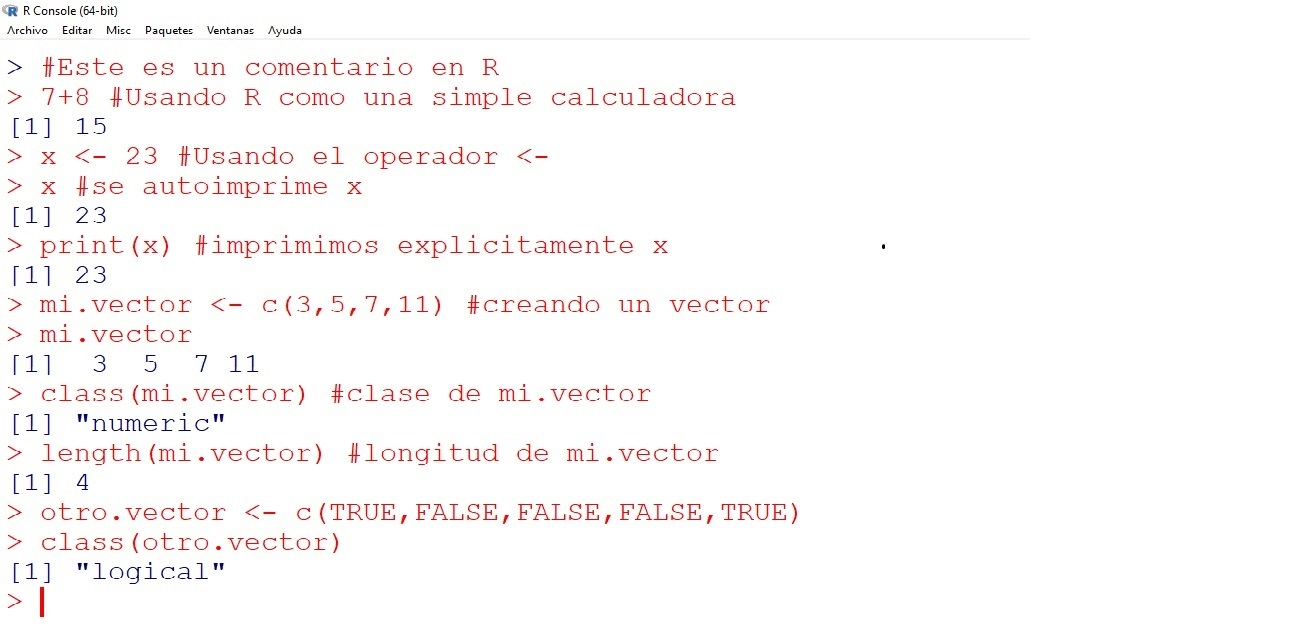
\includegraphics[scale=0.46]{Capitulo3/figs/consola1.jpg}      %Ruta completa de la imagen, porque se compila desde el archivo tesis.tex
  \caption[Entrada de datos en R]{Entrada de datos en R. El [1] que aparece a la izquierda de la salida de la expresión indica que el elemento que se encuentra a la derecha tiene índice 1.}            %Pie de imagen
  \label{consola1}                            %nombre de referencia
\end{figure}


Otros tipos de objetos son las \emph{listas} y los \emph{dataframes}. Una lista, de la clase \emph{list}, es una clase de datos que puede contener elementos de diferentes clases y de distinta longitud o dimensión. Por otro lado, un dataframe es un tipo de dato en R que sirve para guardar datos tabulares donde cada columna representa una variable, las columnas no necesariamente son de la misma clase pero deben tener la misma longitud. Para generar un dataframe se usa \emph{data.frame()}, \emph{read.table()}, \emph{read.csv()}. Ver ejemplos en la Figura \ref{consola2}.\\

\begin{figure}[H]
  \centering
    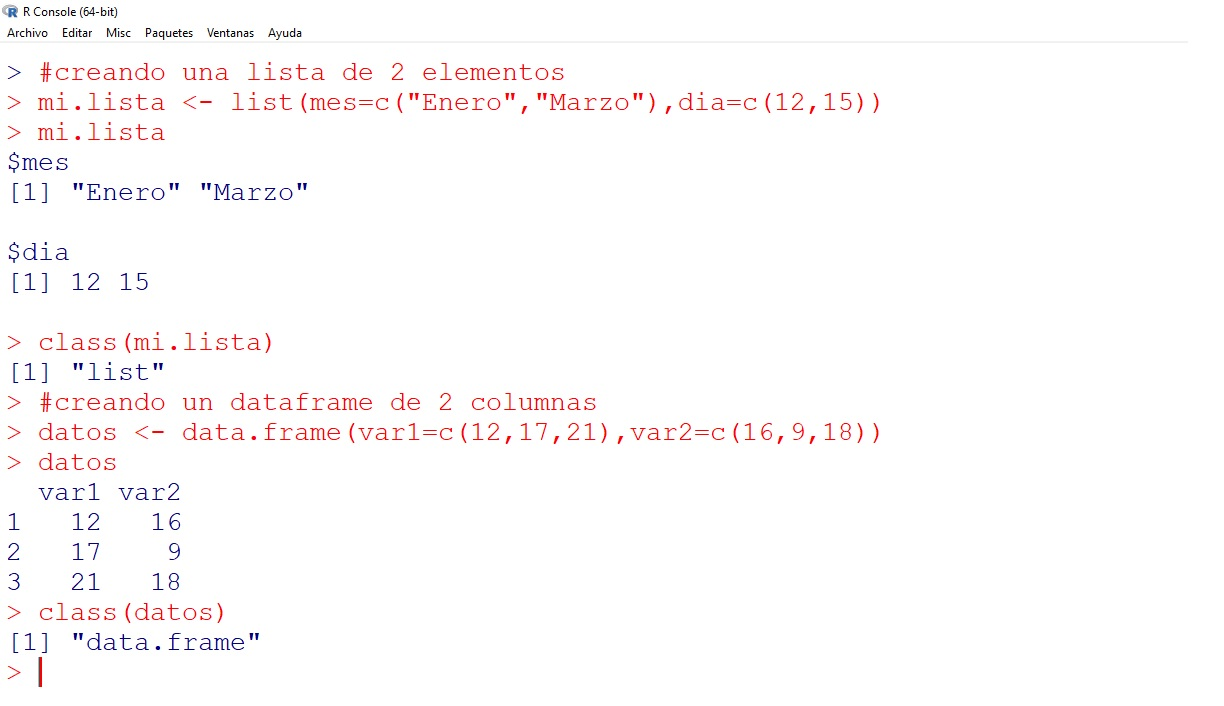
\includegraphics[scale=0.46]{Capitulo3/figs/consola2.jpg}      %Ruta completa de la imagen, porque se compila desde el archivo tesis.tex
  \caption{Creando listas y dataframes.}            %Pie de imagen
  \label{consola2}                            %nombre de referencia
\end{figure}

Para el manejo de fechas y tiempo hay clases especiales dentro del sistema. Este tipo de objetos permiten llevar a cabo operaciones numéricas y estadísticas. Hay un tipo de datos exclusivamente para fechas usando la función \emph{as.Date()}. Además, hay  2 tipos de datos para tiempo: \emph{POSIXct} y POSIXlt. La diferencia entre estos dos es la manera en que almacenan los datos internamente en R, el primero almacena el dato como el número de segundos transcurridos desde el 1 de enero de 1970, mientras que POSIXlt almacena los datos de la fecha y tiempo en forma de lista. \\

Para manipular la información de fecha y tiempo de los datos del TNS se usará la biblioteca \emph{lubridate} porque es más eficiente al hacer la conversión en grandes cantidades de datos  que el paquete base de R. Más adelante se explica detalladamente este procedimiento.\\

En el capítulo 2 se vio cuál es la estructura de los datos, el objetivo de este capítulo es mostrar y explicar a grandes rasgos el código empleado para obtener un dataframe ordenado y el método para hacer la limpieza de datos.

\section{Limpieza y ordenamiento de datos}

La limpieza de datos es una parte esencial del análisis estadístico. De hecho, en la práctica lleva aún más tiempo que el análisis en sí. La limpieza de datos o \emph{data cleaning} es el proceso de transformación de datos crudos en datos consistentes que puedan ser analizados. Si bien el orden de las variables y las observaciones no afectan al análisis, un buen orden hace que sea más fácil que un analista o una computadora extraigan las variables necesarias porque proporciona una forma estándar de estructurar un conjunto de datos.\\

De acuerdo al artículo \textit{Tidy Data} de Hadley Wickham\cite{tidy-data} los datos ordenados deben cumplir con lo siguiente:

\begin{enumerate}
\item Cada variable forma una columna.
\item Cada observación forma una fila. 
\item Cada tipo de unidad observacional forma una tabla.
\end{enumerate}

En esta sección describiré como ordené los datos del TNS de acuerdo a los principios mencionados anteriormente y extrayendo sólo las variables que nos interesan (datos que registran partículas neutras y la fecha y tiempo).\\

El lenguaje R puede leer datos guardados como archivos de texto plano, del tipo \emph{.csv}, \emph{.txt}, \emph{.dat}. También lee archivos en otros formatos (Excel, SAS, SPSS) pero las funciones necesarias no están incluidas en el paquete \emph{base}. Para leer y escribir archivos, R utiliza el directorio de trabajo. Para conocer el directorio se utiliza el comando \emph{getwd()}\footnote{get working directory}. Para cambiar el directorio de trabajo se utiliza la función \emph{setwd()} utilizando como argumento la dirección (path).\\

En el capítulo anterior se comentó que los datos del TNS se guardan en archivos con extension \emph{.sn1}, estos son archivos de texto en formato ASCII que se pueden leer con las funciones \emph{read.table()}, \emph{read.csv()}, \emph{read.csv2()}; las cuales regresan un objeto de tipo \emph{data frame}. Como no es necesario tener el conjunto completo de datos (13 años) todo el tiempo en una sesión de  R, se procesó la información por año.\\ 

Para leer y ordenar los datos del TNS se usaron dos códigos distintos, uno para los datos registrados por minuto y otro para los que se registraron cada 3 y 10 segundos. Estos últimos aún cuando no tengan la misma razón de conteo, los archivos sí tienen la misma estructura por lo que no hay necesidad de tratarlos por separado, ya que en R se pueden hacer operaciones con fechas y tiempos para ponerlos en una misma razón de conteo cuando sea necesario.\\

A continuación se explican los códigos mencionados anteriormente, el primero es un ejemplo para datos de 2005 y el segundo es para el año 2008. Para los demás años se procede de la misma forma que en alguno de los dos casos.\\

Procesamiento de datos para 2005:

Primero se cambia el directorio de trabajo a la carpeta donde se encuentran los archivos de 2005. En la línea 2 se obtienen los nombres de estos archivos y se guarda en la variable ``archivos". En la línea 3 se crea la función \emph{leer1}, ésta recibe un parámetro que se usa en la función \emph{read.table()} y solo va a leer las columnas del 1 al 3 y luego del 5 al 12. En la línea 4, con la función lapply, se aplica la función leer1 con cada una de las entradas del vector archivos, el resultado es una lista con elementos que son dataframes, se guarda en dat05. Por último, en la línea 5 se extrae cada entrada de la lista dat05 y con rbind cada dataframe se ``pega" \, uno debajo de otro. El resultado es un dataframe que contiene todos los datos de 2005 con las columnas del 1 al 3 y del 5 al 12.\\

\begin{mybox}
\begin{Verbatim}[numbers=left,xleftmargin=5mm]
> setwd("./Data_TNS/2005")
> archivos <- list.files()
> leer1 <- function(file){read.table(file)[c(1:3,5:12)]}
> dat05 <- lapply(archivos,leer1)
> dat05 <- do.call(rbind,dat05)
\end{Verbatim}
\end{mybox}

Ya se tienen los datos del año 2005 en un dataframe, falta poner en una sola columna la información de fecha y tiempo para cada observación en el formato año-mes-día hora:minuto:segundo, se hace en el \emph{Paso 2} y \emph{Paso 3}. La primera línea calcula la cantidad de ``ceros" que le falta a cada elemento de la columna 3 para que sean 4 dígitos, y devuelve esa cantidad de ceros en un vector temp. La segunda línea pega el vector temp con la columna 3 de dat05 y otros dos ceros al final, esta operación es elemento a elemento y se ``reescribe" \, en la columna 3. La tercera línea muestra las primeras 4 filas del resultado.\\

Paso 2:
\begin{mybox}
\begin{verbatim}
> temp <- mapply(function(x, y) paste0(rep(x, y), 
	collapse = ""), 0, 4 - nchar(dat05$V3))
> dat05$V3 <- paste0(temp, dat05$V3,00)
> head(dat05,4)
    V1  V2   V3     V5   V6   V7  V8    V9   V10  V11  V12
1 2005 101 000000  9147 3365 1217 561 27783 12932 5109 2476
2 2005 101 000100  9099 3458 1215 574 27809 12872 5039 2446
3 2005 101 000200  8979 3415 1200 526 27854 13016 5014 2415
4 2005 101 000300  8981 3434 1194 573 27917 13013 5079 2484
\end{verbatim}
\end{mybox}

Para el \emph{Paso 3} se instaló previamente la biblioteca \emph{dplyr} (se explica en la siguiente sección), se carga a la sesión de R en la primera línea. La segunda línea es una nueva gramática del paquete dplyr, lo primero que hace es tomar el dataframe dat05, con mutate le agrega una nueva columna llamada \emph{date} que es el resultado de pegar las columnas V1,V2 y V3. Posteriormente, con \emph{select} extrae solo las variables de interés, date y datos de los ocho canales. Luego, con \emph{rename} le pone nombres a las variables. Por último, se muestran las primeras cuatro líneas del resultado y en la última línea guarda el dataframe en una ventana de datos de R, en dat05.RData.\\

Paso 3:
\begin{mybox}
\begin{verbatim}
> library(dplyr)
> dat05 <- dat05 %>% mutate(date = paste(V1,0,V2," ",V3)) %>%
	select(date,V5:V12) %>%
	rename(S1_A=V5,S2_A=V6,S3_A=V7,S4_A=V8) %>%
	rename(S1=V9,S2=V10,S3=V11,S4=V12)
> head(dat05,4)
             date  S1_A S2_A S3_A S4_A  S1    S2   S3   S4 
1 20050101 000000  9147 3365 1217 561 27783 12932 5109 2476
2 20050101 000100  9099 3458 1215 574 27809 12872 5039 2446
3 20050101 000200  8979 3415 1200 526 27854 13016 5014 2415
4 20050101 000300  8981 3434 1194 573 27917 13013 5079 2484
> save(dat05,file="dat05.RData")
\end{verbatim}
\end{mybox}

Ahora véase el ejemplo para el año 2008, el primer paso es igual que el ejemplo anterior, solo difieren en la función \emph{leer2} porque los archivos tienen otra estructura, en este caso  se leerán las columnas del 2 al 11.\\

Ejemplo para datos de 2008.
\begin{mybox}
\begin{Verbatim}[numbers=left,xleftmargin=5mm]
> setwd("./Data_TNS/2008")
> archivos <- list.files()
> leer2 <- function(file){read.csv2(file,header=F,skip=5,sep=" ",
	colClasses=c(rep("character",3),rep("integer",49)))[2:11]}
> dat08 <- lapply(archivos,leer2)
> dat08 <- do.call(rbind,dat08)
\end{Verbatim}
\end{mybox}

El siguiente paso es similar al Paso 3 del ejemplo anterior. Se toma el dataframe dat08, con mutate se le agrega la columna date y con select se extraen las columnas date y datos de los ocho canales. Al final se guarda el dataframe en la ventana de datos \emph{dat08.RData}.\\

Paso 2:
\begin{mybox}
\begin{verbatim}
> library(dplyr)
> data08 <- dat08 %>% mutate(date = paste(V2,V3)) %>%
	select(date,V4:V11) %>%
	rename(S1_A=V4,S2_A=V5,S3_A=V6,S4_A=V7) %>%
	rename(S1=V8,S2=V9,S3=V10,S4=V11)
> save(dat08,file="dat08.RData")
\end{verbatim}
\end{mybox}

Como se ha mencionado anteriormente, hay varios paquetes que se han desarrollado para complementar el lenguaje de R. Si bien muchos paquetes desarrollan nuevos algoritmos, hay otros que realizan acciones que se pueden llevar a cabo con el paquete base. La ventaja de estas bibliotecas es que reducen el tiempo de ejecución cuando se trabaja con grandes cantidades de datos y el lenguaje es más intuitivo, por ejemplo \emph{lubridate} y \emph{dplyr}.\\ 

Hasta este punto se tienen los datos ordenados del TNS para cada año y todos tienen la misma estructura, pero falta ``decirle" \, a R que la columna \emph{date} de cada dataframe es una columna de fechas y tiempo. Para convertir esta columna en clase ``date/time" se usará la biblioteca \emph{lubridate}, el código se muestra en la siguiente sección así como una breve descripción de los paquetes que permitieron trabajar los datos del TNS de manera eficiente.\\

\section{Paquetes usados de R}
Para usar los paquetes que no están incluidos en el \emph{paquete base} es necesario instalarlos. Para ello se usa la función \emph{install.packages()} con argumento entre comillas la biblioteca que se desea instalar. Después con la función \emph{library()} se carga la biblioteca al área de trabajo.

Ejemplo:
\begin{mybox}
\begin{verbatim}
>install.packages("dplyr")
>library(dplyr)
\end{verbatim}
\end{mybox}

A continuación se describen algunos paquetes en el orden en que fueron utilizados para llevar a cabo este trabajo.\\


\subsection{dplyr}
dplyr es una nueva gramática de manipulación de datos, una herramienta rápida, flexible y consistente para trabajar con datos como objetos. Entre las funciones más importantes se encuentran \emph{mutate},\emph{select}, \emph{rename}, \emph{filter}, \emph{arrange} y \emph{$group\_by$} \cite{dply}. Estas funciones fueron muy útiles al procesar los datos, como se vio en los ejemplos anteriores, ya que reduce el tiempo de ejecución comparado con las funciones que realizan la misma acción en el paquete base. Además el lenguaje es más claro y reduce líneas de código.

\subsection{lubridate}

Lubridate es un paquete de R, creado por Garrett Grolemund y Hadley Wickham, que hace mucho más fácil el trabajo con datos de fechas y horas. Identifica el orden en que aparece el año, mes y día en los datos. Además de que facilita el trabajo con zonas horarias, por defecto lubridate pone la fecha en tiempo universal (TU). En el link se pueden ver ejemplos de las herramientas que ofrece este paquete: \url{https://cran.r-project.org/web/packages/lubridate/vignettes/lubridate.html} o bien en \textit{Dates and times made easy with lubridate} de Garrett Grolemund y Hadley Wickham\cite{lubrid}.\\

Se usará esta biblioteca  para convertir a clase POSIXct la columna \emph{date} de cada tabla de datos del TNS. Como estas tablas ya tienen la misma estructura el siguiente código funciona para todas. Lo primero que se hace es localizar los índices de los datos que se registraron en horario de verano y los que no, de acuerdo a estos índices se crea un vector que contiene  CDT (Central Daylight Time) si el dato corresponde al horario de verano y  CST (Central Standard Time) si no (esta parte se trabajó de manera interactiva localizando las fechas del cambio de horario).\\ 

En el siguiente ejemplo primero se carga la bibioteca lubridate. En la segunda línea, la función \emph{merge} junta dat05 con el dataframe que tiene por columnas TZONE y OFFSET. Si la observación tiene asignado el caracter $\mathrm{``CDT"}$, en la columna OFFSET del dataframe dat05 se le asigna $-5$ y se le asigna $-6$ si tiene $\mathrm{``CST"}$.\\

Ejemplo para \emph{dat05}
\begin{mybox}
\begin{Verbatim}[numbers=left,xleftmargin=5mm]
> library("lubridate")
> data05 <- merge(dat05, data.frame(TZONE = c("CDT", "CST"), 
 	 OFFSET = c(-5, -6)))
> data_1$DATE_UTC <- ymd_hm(data_1$date, 
	 tz = "UTC") - dhours(data_1$OFFSET)
> data_1$DATE_LOCAL <- with_tz(data_1$DATE_UTC, "America/Mexico_City")
> data_1<- data_1[order(data_1$DATE_UTC), ]
\end{Verbatim}
\end{mybox}

En la cuarta línea se convierte la columna \emph{date} a clase POSIXct pero en Tiempo Universal (UTC), por lo que se le suma la cantidad de horas que faltan, estas horas se encuentran en la columna OFFSET. En la quinta línea, con la función  \emph{with\_tz} la columna DATE\_UTC se cambia a la zona horaria de $\mathrm{``America/Mexico\_City"}$, a tiempo local, y finalmente se ordenan los datos de acuerdo a la hora.\\

Es necesario convertir las fechas y horas primero en tiempo universal y despues a tiempo local, ya que si se hace lo último directamente se producen NA's en las horas repetidas, lo cual hace que la serie sea discontinua cuando si se tiene información de esos datos.

Una vez que se tuvieron los datos ordenados se procedió con la limpieza. Esta parte se trabajó de manera interactiva, explorando cómo se distribuyen los datos y detectando los valores atípicos.\\

Se observó que al procesar la información, las variables de partículas cargadas no se eliminaron. Esto debido a que se encontraron errores en el registro, había observaciones para las cuales los datos de partículas neutras eran exactamente igual a los datos de partículas cargadas, es decir, el dato del canal S1\_A igual al S1, el S2\_A igual al S2 y así hasta el S4\_A igual al S4. Además, estos datos estaban en el rango de las variables de partículas cargadas, así que se eliminaron esos índices.\\

Los ceros y datos que se repetían durante varios minutos en todos los canales se sustituyeron por NA (Not Available), que es la forma en que se denotan los valores faltantes en R, ya que era evidente que se trataba de errores electrónicos.\\

También era fácil ver que se trataba de errores aquellos datos que incrementaban y disminuían repentinamente hasta un 20\% con respecto al dato anterior y posterior. Al hablar de estabilidad de datos, lo que se busca es que la variación sea pequeña. En caso de encontrar alguna variación significativa investigar qué pudo haber afectado la toma de datos. Cuando ya no eran tan evidentes los errores se tenía que graficar la serie para ver si había variaciones importantes. Para esto, fue de mucha utilidad el siguiente paquete.

\subsection{Openair}

La biblioteca Openair está diseñada para hacer análisis de datos de calidad del aire, sin embargo ofrece herramientas muy utiles para hacer análisis de variación en series de tiempo, sobretodo la función para agregar datos en distintos intervalos de tiempo. Es por ello que se escogió este paquete para trabajar los datos del TNS. Se puede ver más acerca del paquete en \emph{openair --- An R package for air quality data analysis}\cite{openair} y en \emph{Lenguaje R aplicado al análisis de Calidad de Aire}\cite{manualOp}.\\

Para hacer las gráficas de variación del capítulo 4 se creó la función \emph{variacion} que recibe dos argumentos, el primero es el dataframe y el segundo es el canal que se desea graficar. Luego estos parámetros se usan en la función timeVariation de openair.

\begin{mybox}
\begin{verbatim}
> library("openair")
> variacion <- function(datos,canal){
	timeVariation(datos, pollutant=canal,
	main="Variación temporal del flujo de partículas neutras",
	xlab=c("Flujo horario durante la semana","Flujo horario",
	"Flujo mensual","Variación por días de la semana"))
	}
\end{verbatim}
\end{mybox}

Así, para hacer una gráfica de variación de los datos de 2005 del canal S1\_A se hace de la siguiente forma.
\begin{mybox}
\begin{verbatim}
> variacion("dat05","S1\_A")
\end{verbatim}
\end{mybox}

Hasta este punto se ha cumplido el objetivo de tener datos ordenados y que la fecha y hora de éstos sea  reconocida como tal en R, además se limpiaron los datos de partículas neutras que eran igual a los datos de partículas cargadas. Luego se extrajeron solo la columna date y datos de los cuatro canales de interés.  A partir de aquí se empezaron a localizar los valores atípicos y ver si se debían a errores electrónicos. Sin embargo, había casos en los que el intervalo de errores era demasiado grande y por eso los datos ``correctos" eran los que se mostraban fuera de rango. Como en el caso de los datos de 2008, hasta que se graficaron los datos se observó su comportamiento. Véase el siguiente capítulo para ver las gráficas de variación por año. 



